%%%%%%%%%%%%%%%%%%%%%%%%%%%%%%%%%%%%%%%%%%%%%%%%%%%%%%%%%%%%%%%%%%%%%%%%%%%%%%%%%%%%%%%%%%%%%%%%%%%%%%%%%
%%%%%%%%%%%%%%%%%%%%%%%%%%%%%%%%%%%%%%%%%%%% Header %%%%%%%%%%%%%%%%%%%%%%%%%%%%%%%%%%%%%%%%%%%%%%%%%%%%%
%%%%%%%%%%%%%%%%%%%%%%%%%%%%%%%%%%%%%%%%%%%%%%%%%%%%%%%%%%%%%%%%%%%%%%%%%%%%%%%%%%%%%%%%%%%%%%%%%%%%%%%%%

\documentclass[a4paper,titlepage,11pt,twosides,floatssmall]{mwrep}

\usepackage[left=2.5cm,right=2.5cm,top=2.5cm,bottom=2.5cm]{geometry} % Pages' geometry and layout
\usepackage{amsmath} % Mathematical commands
\usepackage{amsfonts} % Fonts commands
\usepackage{amssymb} % Symbolical commands
\usepackage[T1]{fontenc} % Defines encoding for fonts (OT1 - original TeX encoding) 
\usepackage[polish]{babel} % Polish language specifics
\usepackage{graphicx} % Importing external graphics
\usepackage{float} % Forcing plot's position
\usepackage{url} % Web-related text (urls, mail adresses, etc.)
\usepackage{tikz} % Creating graphical elements like lines, dots, curves, figures
\usepackage{rotating} % Rotating objects of an arbitrary angle
\usepackage[percent]{overpic} % Makes it able to put LaTeX commands onto the included graphics (with a dedicated environment)
\usepackage[utf8]{inputenc} % Non-standrard encoding of the LaTeX files
\usepackage{xcolor} % Easy driver-independent access to several kinds of color tints, shades, tones, and mixes of arbitrary colors
\usepackage{pgfplots} % High-quality function plots in normal or logarithmic scaling with a user-friendly interface
\usepackage{listings} % Source code printer
\usepackage{matlab-prettifier} % Matlab source code printer
\usepackage{enumitem} % List environments
\usepackage{siunitx} % Physical units
\usepackage{float} % force figure anchoring
\usepackage[nottoc]{tocbibind}

% tikz packages choice
\usetikzlibrary{arrows,calc,decorations.markings,math,arrows.meta}
\usetikzlibrary{pgfplots.groupplots}

% siunitx settings
\sisetup{detect-weight,exponent-product=\cdot,output-decimal-marker={,},per-mode=symbol,binary-units=true,range-phrase={-},range-units=single}
\SendSettingsToPgf % unifies settings of the pgfplots package with siunitx package

% listings settings
\definecolor{gray}{rgb}{0.95,0.95,0.95}
\lstset{
	backgroundcolor=\color{gray},
	frame=single,
	breaklines=true,
}

% listings styles
\lstdefinestyle{customlatex}{
	basicstyle=\footnotesize\ttfamily,
	% basicstyle=\small\ttfamily,
}
\lstdefinestyle{customc}{
	breaklines=true,
	frame=tb,
	language=C,
	xleftmargin=0pt,
	showstringspaces=false,
	basicstyle=\small\ttfamily,
	keywordstyle=\bfseries\color{green!40!black},
	commentstyle=\itshape\color{purple!40!black},
	identifierstyle=\color{blue},
	stringstyle=\color{orange},
}
\lstdefinestyle{custommatlab}{
	captionpos=t,
	breaklines=true,
	frame=tb,
	xleftmargin=0pt,
	language=matlab,
	showstringspaces=false,
	% basicstyle=\footnotesize\ttfamily,
	basicstyle=\scriptsize\ttfamily,
	keywordstyle=\bfseries\color{green!40!black},
	commentstyle=\itshape\color{purple!40!black},
	identifierstyle=\color{blue},
	stringstyle=\color{orange},
}

% Text field size (without header and footer - bez "¿ywej paginy")
\textwidth 160mm \textheight 247mm

% pgfplots settings
\pgfplotsset{
	tick label style={font=\scriptsize},
	label style={font=\small},
	legend style={font=\small},
	title style={font=\small}
}

\addto\captionspolish{\renewcommand{\figurename}{Rys.}}
\addto\captionspolish{\renewcommand{\tablename}{Tab.}}

% Max number of floating elements configuration
\setcounter{topnumber}{0} % default : 2
\setcounter{bottomnumber}{3} % default : 1
\setcounter{totalnumber}{5} % default : 3

\renewcommand{\textfraction}{0.01} % default : 0.2
\renewcommand{\topfraction}{0.95} % default : 0.7
\renewcommand{\bottomfraction}{0.95} % default : 0.3
\renewcommand{\floatpagefraction}{0.35} % default : 0.5

% Path to the graphics
\graphicspath{ {./img/} }

%%%%%%%%%%%%%%%%%%%%%%%%%%%%%%%%%%%%%%%%%%%%%%%%%%%%%%%%%%%%%%%%%%%%%%%%%%%%%%%%%%%%%%%%%%%%%%%%%%%%%%%%%
%%%%%%%%%%%%%%%%%%%%%%%%%%%%%%%%%%%%%% Document utilities %%%%%%%%%%%%%%%%%%%%%%%%%%%%%%%%%%%%%%%%%%%%%%%
%%%%%%%%%%%%%%%%%%%%%%%%%%%%%%%%%%%%%%%%%%%%%%%%%%%%%%%%%%%%%%%%%%%%%%%%%%%%%%%%%%%%%%%%%%%%%%%%%%%%%%%%%

% Title Page Data
\title{\bf Neuroewolucja - gra w gre \vskip 0.1cm}
\author{Kacper Kula, Krzysztof Pierczyk}
\date{czerwiec 2020}

% Maketitle macro
\makeatletter
\renewcommand{\maketitle}
{
	\begin{titlepage}
		\begin{center}{
			\LARGE {\bf
			Wydział Elektroniki i Technik Informacyjnych}}\\
			\vspace{0.4cm}
			{\LARGE {\bf Politechnika Warszawska}}\\
			\vspace{0.3cm}
		\end{center}
		\vspace{5cm}
		\begin{center}
            {\bf \LARGE Algorytmy Heurystyczne \vskip 0.1cm}
            {\bf \LARGE \@title}
		\end{center}
		\vspace*{\stretch{6}}
        \begin{center}
            {\bf \Large \@author \par}
			\bf{\large{Warszawa, \@date\vskip 0.1cm}}
		\end{center}
	\end{titlepage}
}
\makeatother

%%%%%%%%%%%%%%%%%%%%%%%%%%%%%%%%%%%%%%%%%%%%%%%%%%%%%%%%%%%%%%%%%%%%%%%%%%%%%%%%%%%%%%%%%%%%%%%%%%%%%%%%%
%%%%%%%%%%%%%%%%%%%%%%%%%%%%%%%%%%%%%%%%%%% Document %%%%%%%%%%%%%%%%%%%%%%%%%%%%%%%%%%%%%%%%%%%%%%%%%%%%
%%%%%%%%%%%%%%%%%%%%%%%%%%%%%%%%%%%%%%%%%%%%%%%%%%%%%%%%%%%%%%%%%%%%%%%%%%%%%%%%%%%%%%%%%%%%%%%%%%%%%%%%%

\begin{document}

% Pages' style formatting
\frenchspacing
\pagestyle{uheadings}

% Use maketitle macro to build title page
\maketitle

% Insert parts of the report
\tableofcontents
\chapter{Wprowadzenie}

Inspiracje biologiczne są obecne w~inżynierii już od wielu lat. Możemy się na nie natknąć nie tylko w~mechanice, awionice czy rbotyce. Zagrzały one miejsce również wśród szeroko rozumianych metod sztucznej inteligencji (ang. \textit{Artificial Intelligence, AI}). Jedną z~najciekawszych inspiracji na tym polu wydają sie być sztuczne sieci neuronowe (ang. \textit{Artificial Neural Networks, ANN}). Ich koncepcja pojawiła się już w połowie XX wieku \cite{perceptron}, jednak brak teoretycznych podstaw, które umożliwiałyby efektywne uczenie sieci sprawi, że nie zyskały one popularności w~następnych latach. Dopiero zaproponowana w~1986 metoda wstecznej propagacji błędu \cite{backprop} spowodowała powrót do koncepcji ANN szerszego grona badaczy. Dynamiczny wzrost mocy obliczeniowej komputerów oraz wypracowanie solidnych podstaw teoretycznych sprawiły, że sztuczne sieci neuronowe są dzisiaj jednym z~głównych narzędzi sztucznej inteligencji, które wykorzystywane jest w~badaniach naukowych, analizach rynku czy szeroko pojętym modelowaniu.

\section*{Opis projektu}

Chociaż algorytmy oparte na wstecznej propagacji błędu stanowiły przez lata oś zainteresowania w~kwestii uczenia ANN okazują się one nie być jedynymi dostępnymi. Celem naszego projektu było zaimplementowanie alternatywnych metod uczenia opartych o~mechanizmy znane z~algorytmów ewolucyjnych, sprawdzenie ich wydajności oraz porównanie z podejściem klasycznym na bazie gier znanych z~konsoli Atari. Jako środowisko testowe posłużyła nam otwarta biblioteka \textit{OpenAI Gym} dostępna w języku Python. Poprzez prosty interfejs udostępnia ona szerek ujednoliconych środowisk testowych umożliwiających testowanie algorytmów uczenia ze wzmocnieniem. Spośród nich wybraliśmy emulację gry Breakout (w~wersji ze stanem reprezentowanym przez pamięć RAM gry).  Klasyczne wykorzystanie sieci neuronowych kojarzy się raczej z~uczeniem nadzorowanym, którego zadaniem jest budowa modelu potrafiącego przypisać danym wejsciowym jedną z~dostępnych etykiet. Istnieją jednak metody uczenia, które pozwalają wykorzystać sieci równiez w~zadaniach uczenia ze wzmocnieniem. Właśnie jedeną z takich metod - \textit{Deep Q Learning} - wykorzystaliśmy jako punkt odniesienia dla podejścia ewolucyjnego.

\begin{figure}
    \centering
    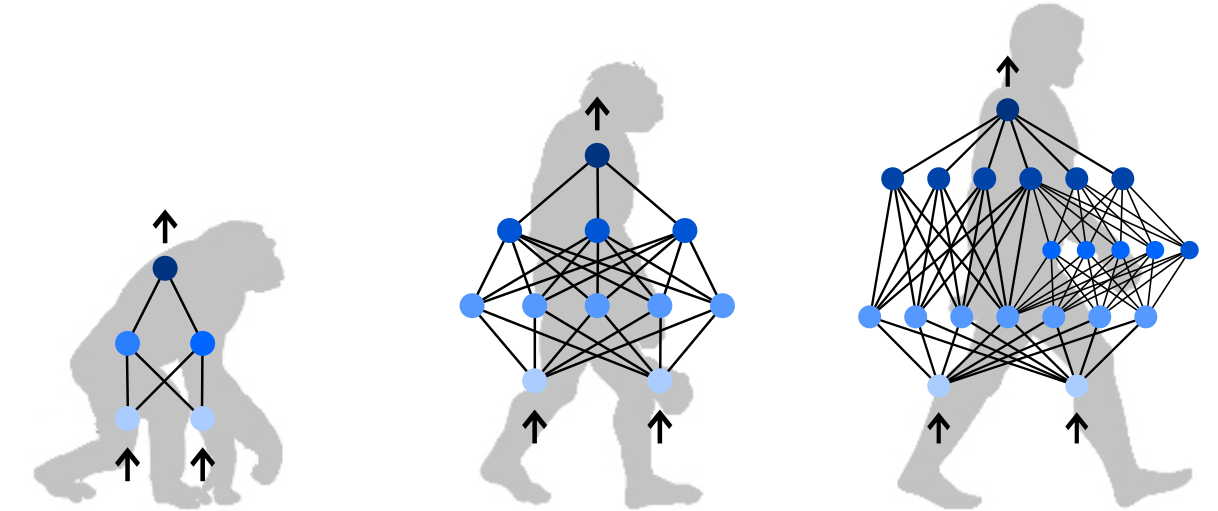
\includegraphics[scale=0.3]{neuroevolution.png}
    \caption{Poglądowe spojrzenie na neuroewolucję}
    \label{neuroevolution}
\end{figure}

Jednym z~największych problemów stojących przed projektantem sztucznej sieci neuronowej jest odpowiedni dobór hiperparametrów takich jak ilość wartw czy ilość neuronów w~poszczególnych warstwach. Dzięki wykorzystaniu mechanizmów ewolucyjnych możliwe jest stworzenie algorytmów, które poza parametrami sieci dostosowują również w~dynamiczny sposób jej topologię. W~ramach projektu zdecydowaliśmy się zbadać zarówno metody o~stałej jak i~o~zmiennej topologii co dobprowadziło do wyróżnienia czterech rónych wariantów uczenia:

\vskip 0.5cm
\begin{itemize}[leftmargin=1cm]
    \item[$\bullet$] uczenie sieci o~stałej topologii z~wykorzystaniem wstecznej propagacji błędu
    \item[$\bullet$] uczenie sieci o~stałej topologii z~wykorzystaniem algorytmu ewolucyjnego
    \item[$\bullet$] uczenie sieci o~zmiennej topologii dostosowywanej przez algorytm ewolucyjny; dobór wag metodą wstecznej propagacji błędu
    \item[$\bullet$] uczenie sieci o~zmiennej topologii dostosowywanej przez algorytm ewolucyjny; dobór wag metodą ewolucyjną
\end{itemize}
\vskip 0.5cm
\chapter{Podejście klasyczne}

Aby wyznaczyć punkt odniesienia dla badań związanych z~neuroewolucją rozpoczęliśmy od uczenia naszej sieci metodą wstecznej propagacji błędu. Pomysł na wykorzystanie jej w~uczeniu ze wzmocnieniem nie przychodzi w~tak oczywisty sposób jak w~przypadku uczeni nadzorowanego. Z~tego wzlędu postanowiliśmy przyjrzeć się głębiej naturze samego problemu.

\section*{Uczenie ze wzmocnieniem}

Uczenie ze wzmocnieniem (ang. \textit{Reinforcement Learning, RL})jest to dziedzina uczenia maszynowego zajmująca się metodami wyznaczania optymalnej strategii zachowania agenta w~nieznanym mu środowisku. Celem agenta jest maksymalizacja nagrody otrzymywanej za interakcję ze środowiskiem. środowisko modeluje się najczęciej jako proces decyzyjny Markova (ang. \textit{Markov decission process, MDP}), który można przedstawić jako krotkę podstaci

\begin{equation}
    <S,A,P_a(s, s'),R_a(s, s'),O>
\end{equation}

gdzie $S$ - zbiór wszystkich stanów agenta i~środowiska, $A$ - zbiór akcji możlwiwych do podjęcia przez agenta, $P_a(s, s')$ - prawdopodobieństwo przejścia ze stanu $s$ do stanu $s'$ pod wplywem akcji $a$, $R_a(s, s')$ - natychmiastowa nagroda przy przejściu ze stanu $s$ do stanu $s'$ pod wpływem akcji $a$, $O$ -  zasady opisujące obserwacje agenta. Agent oddziałuje z~otoczeniem w~dyskretnych chwilach. W~każdej chwili $t$ otrzymuje on obserację $o_t$ i~nagrodę $r_t$ (zazwyczaj w~postaci wartości skalarnej) oraz decyduje się na podjęcie akcji $a_t$. Proces ten został poglądowo przedstawiony na \figurename\ref{reinforcement-learning}

\vskip 0.5cm
\begin{figure}[h]
    \centering
    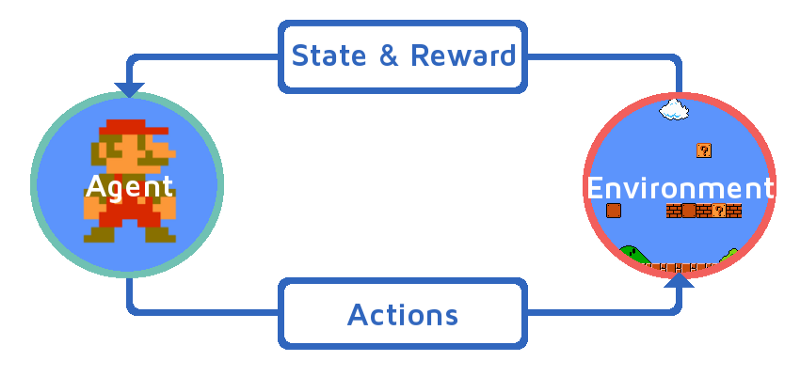
\includegraphics[scale=0.3]{reinforcement_learning_loop.png}
    \caption{Typowy schemat interakcji agenta ze środowiskiem}
    \label{reinforcement-learning}
\end{figure}
\vskip 0.5cm

Model podejmowania decyzji przez agenta nazywa się polityką (ang. \textit{policy}) i~można go przedstawić w~podstaci \ref{policy}. Polityka określa prawdopodobieństwo podjęcia przez agenta akcji $a$ w~stanie $s$.

\vskip 0.5cm
\begin{equation}
\begin{cases}
    \pi: A \times S \rightarrow [0,1] \\
    \pi(a,s) = P\left\{a_t = a | s_t = s\right\} 
    \label{policy}
\end{cases}
\end{equation}
\vskip 0.5cm

Aby ocenić jakość stanu agent dysponuje funkcją wartości stanu (ang. \textit{state-value function}) postaci widocznej na \ref{state-value-function}, gdzie $\gamma$ jest skalarem z przedziału $[0, 1]$. Zwraca ona wartość oczekiwaną sumy przyszłych nagród wziętych z~odpowiednimi wspóczynnikami oznaczaną przez $R$.

\vskip 0.5cm
\begin{equation}
    V_{\pi}(s) = E\left[\sum_{t=0}^{\infty} \gamma^tr_t | s_0=s\right] = E\left[R|s=s_0\right]
    \label{state-value-function}
\end{equation}
\vskip 0.5cm

Funkcja wartości polityki(ang. \textit{value function}) jest z~kolei metodą określenia jakości całego mechanizmu decyzyjnego. Analogicznie do funkcji wartości stanu jest ona zdefiniowana jako wartość oczekiwana ważonej sumy przyszłych nagród dla stanu $s$ przy wykorzystaniu polityki $\pi$. Ukazano ją na \ref{policy-value-function}.

\vskip 0.5cm
\begin{equation}
    V^{\pi}(s) = E\left[R|s, \pi\right]
    \label{policy-value-function}
\end{equation}
\vskip 0.5cm

Definicja ta pozwala nam zdefiniować optymalną politykę jako tę, która maksymalizuje swoją wartość $V^{\pi}$ niezależnie od wybranego stanu $s$. Chociaż definicja ta jest wystarczająca, często definiuje się dodatkowy element nazywany funkcją wartości akcji (ang. \textit{action-values function}). Jest ona postaci \ref{action-values-function} i~określa oczekiwaną wartość ważonej sumy przyszłych nagród w~sytuacji, w~której agent, znajdując sie w~stanie $s$ wykonał akcję $a$, a~następnie działał zgodnie z polityką$\pi$.

\vskip 0.5cm
\begin{equation}
    Q^{\pi}(s,a) = E[R|s, a, \pi]
    \label{action-values-function}
\end{equation}
\vskip 0.5cm

Algorytmy uczenia ze wzmocnieniem są budowane na dwa sposoby. Pierwszy to bezpośrednia próba odnalezienia polityka $\pi(s)$, czyli modelu, który widząc na wejściu stan $s$ zwraca optymalną akcję $a$. Drugie podejście modeluje nie samą politykę, a~funkcję $Q^{\pi}(s, a)$. Z~definicji tej funkcji wynika, że jeżeli ${\pi}^*$ jest polityką optymalną, to agent moze postępować optymalnie poprzez wybieranie tej akcji ze zbioru ${Q^{\pi^*}(s, a) : a \in A}$, której wartość jest największa - nie wymaga od nas znajomości samej polityki $\pi^*$. To na pozór trywialne spostrzeżenie, zwane \textit{równaniem Bellmana}\cite{bellman} pozwala na budowę efektywnych algorytmów uczenia, których przykładem jest wybrany przez nas \textit{Deep Q Network} (DQN). 


\section*{Deep Q Network}

Q-learning jest algorytmem uczenia ze wzmocnieniem bazującym na estymacji funkcji $Q(s,a)$ (stąd nazwa). Estymowana funkcja pozwala agentowi podejmować suboptymalne decyzje poprzez wybór tej z~nich, która maksymalizuje jej wartość. Wartości $Q$ są aktualizowane wraz z kolejnymi obserwacjami. Wzór na aktualizację bazuje na równaniu Bellmana i ma postać \ref{q-learning}

\vskip 0.5cm
\begin{equation}
    Q^{t+1}(s_t, a_t) = Q^{t}(s_t, a_t) + \alpha \times \left[r_t + \gamma \times \max_a Q^{t}(s_{t+1}, a_{t+1}) - Q(s_t, a_t)\right]
    \label{q-learning}
\end{equation}
\vskip 0.5cm

Sieć aproksymująca posiada liczbę wejść równą liczbie zmiennych opisujących stan układu, natomiast liczb wyjść jest równa liczbie możliwych do podjęcia przez agenta akcji. Każde z~wyjść opisuje zatem wartość jednej z~tych akcji w~stanie podanym na wejściu. Stosując równanie \ref{q-learning} do takiej sieci uzyskujemy funkcję błędu postaci \ref{cost-function}

\vskip 0.5cm
\begin{equation}
    c(s) = E\left[\|(r_{t} + \gamma \times \max_{a_{t+1}}Q^{t}(s_{t+1},a_{t+1}))-Q^{t}(s,a)\|\right]
    \label{cost-function}
\end{equation}
\vskip 0.5cm

\section*{Implementacja}

Implementacja DQN została w~dużej części zaczerpnięta z~\cite{live-lessons}. Jak już wcześniej wspomniano, poligonem testowym była dla nas gra Breakout, jednak sam program został stworzony tak, aby umożliwić wykorzystanie dowolnego środowiska udostepnianego przez \textit{OpenAI Gym}. Agent jest inicjalizowany losowymi wagami. W~kolejnych iteracjach wykonuje on akcje, dla których przewidywana wartość skumulowanej nagrody jest największa. Korelacja między kolejnymi obserwacjami może sprawić, że sieć będzie niestabilna. Aby temu zapobiec krotki postaci \ref{learning-data-dqn}

\vskip 0.5cm
\begin{equation}
    <s_t, a_t, r_t, s_{t+1}>
    \label{learning-data-dqn}
\end{equation}
\vskip 0.5cm

są zapisywane w~dedykowanej tablicy. Po zakończeniu podejścia do gry zostaną one wykorzystane w~procesie uczenia. Zmniejszenie korelacji następuje poprzez losowy wybór próbek z~zapisanego zbioru. Ilość próbek wykorzystana w~pojedynczej iteracji STG (ang. \textit{Stochastic Gradient Descend}) jest jednym z~parametrów algorytmu. Obszar pamięci, w~którym zapisywane są dane uczące stanowi kolejkę o~ograniczonej pojemności. Jeżeli się ona przepeni, to nowe dane wstawiane są na początku kolejki, natomiast najstarsze dane zostją usunięte. Aby kontrolować tendencje algorytmu do eksplorowania przestrzeni wprowadzony został również parametr $\epsilon \in [0,1]$. Gdy ma on niezerową wartość istnieje szansa, że agent wykona losową akcję zamiast tej przewidzianej przez sieć. Parametr ten jest inicjalizowany niezerową wartością i~zmniejszany wraz przebiegiem uczenia.


\bibliography{bibliography}
\bibliographystyle{plain}

\end{document}